\documentclass[border=10pt]{standalone}

\usepackage{tikz}
\usepackage{tikzsymbols}
\usetikzlibrary{calc,patterns,shapes.geometric}

\def\centerarc[#1](#2)(#3:#4:#5){\draw[#1] ($(#2)+({#5*cos(#3)},{#5*sin(#3)})$) arc (#3:#4:#5);}

\begin{document}
	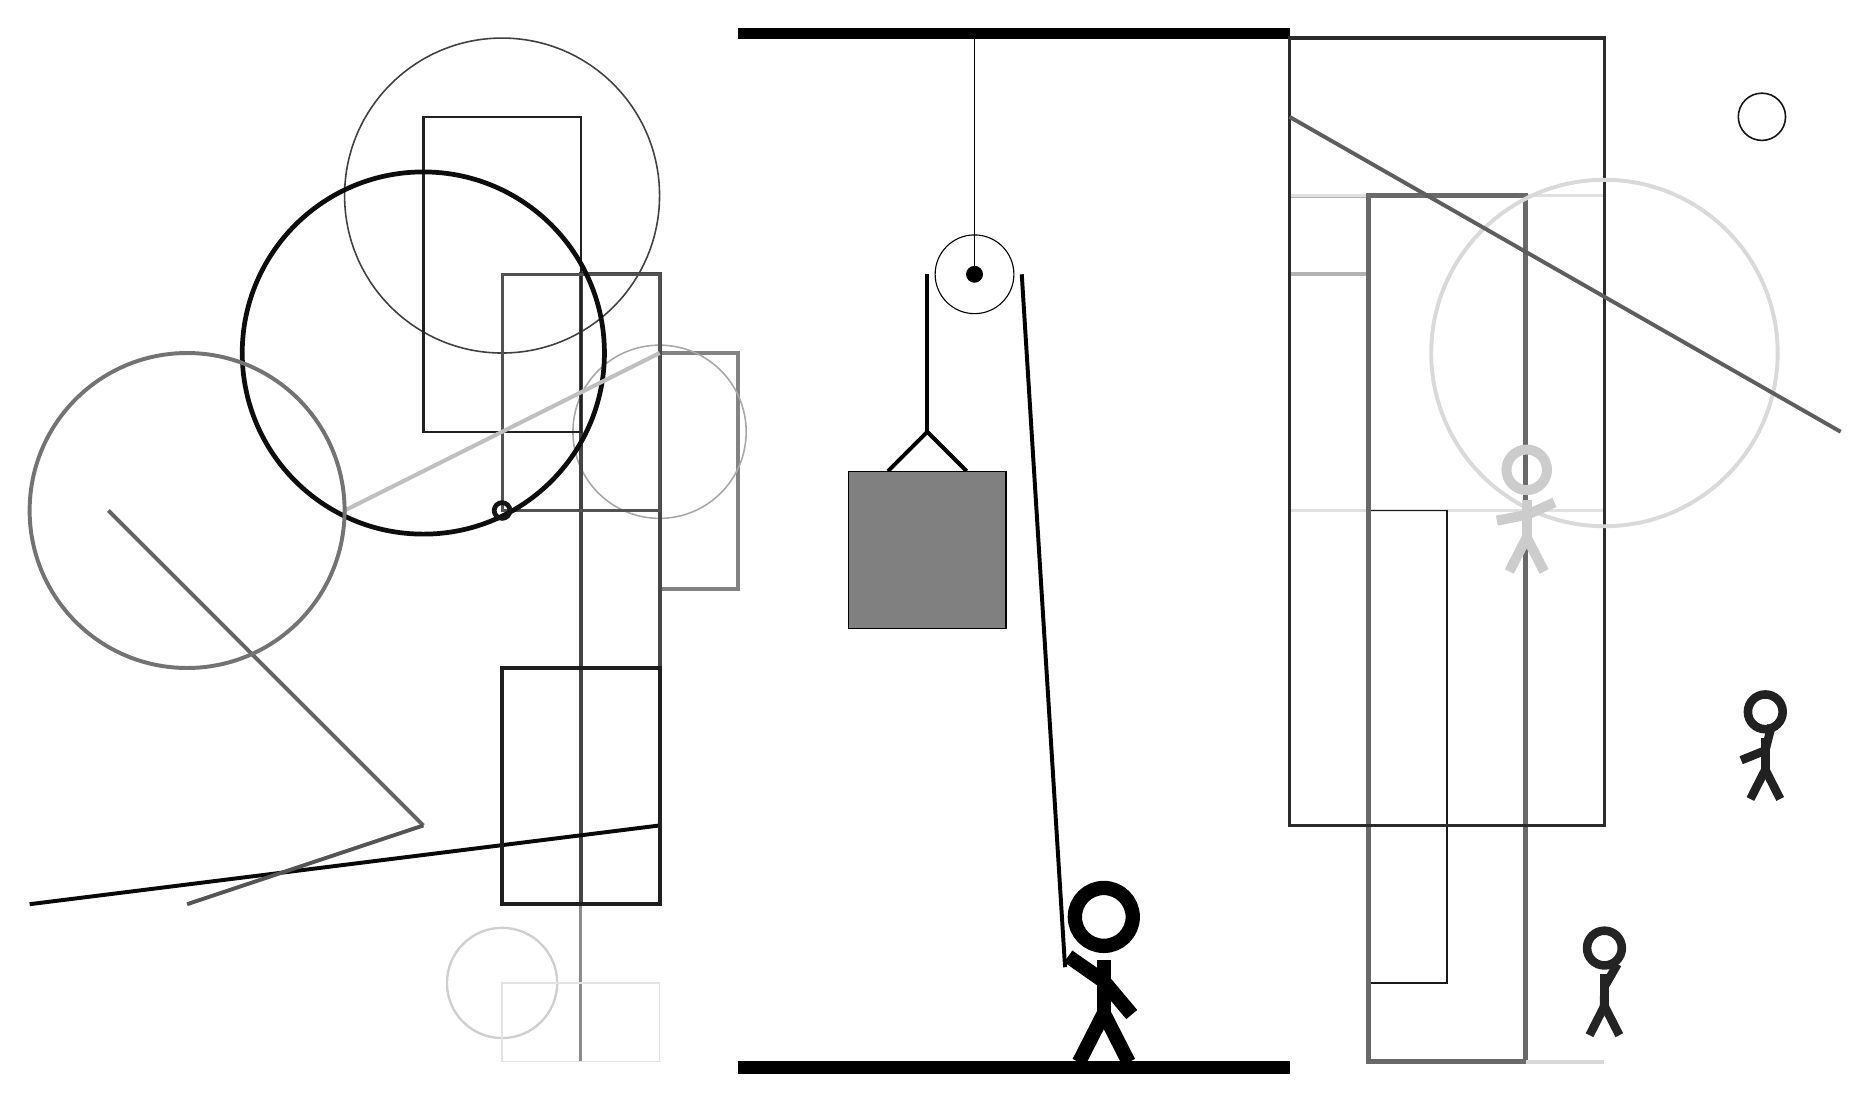
\begin{tikzpicture}
		%%%%% START %%%%%
		
		\draw[fill=black] (-2, 10) rectangle (5, 10.125);
		
		\draw[line width=0.5mm, color=black!49] (-3, 6) rectangle (-2, 3);
		
		\draw[line width=0.5mm, color=black!30] (6, 8) rectangle (5, 7);
		\draw[line width=0.4mm, color=black!45] (-4, 1) rectangle (-4, -3);
		\draw [line width=0.2mm, color=black!34](-3, 5) circle (1.1);
		\draw[line width=0.5mm, color=black!73] (-4, -1) rectangle (-3, 7);
		\draw [line width=0.2mm, color=black!75](-5, 8) circle (2.0);
		
		\draw[line width=0.3mm, color=black!87] (-4, 9) rectangle (-6, 5);
		
		\draw[line width=0.4mm, color=black!68] (-3, 4) rectangle (-5, 7);
		\draw[line width=0.3mm, color=black!12] (5, 8) rectangle (9, 4);
		
		\draw[line width=0.4mm, color=black!89] (6, 8) rectangle (6, -2);
		
		\draw [line width=0.6mm, color=black!95](-6, 6) circle (2.3);
		
		\draw[line width=0.5mm, color=black!61](-6, 0) -- (-10, 4);
		\draw[line width=0.2mm, color=black!90] (6, -2) rectangle (7, 4);
		
		\draw [line width=0.3mm, color=black!19](-5, -2) circle (0.7);
		\node[line width=0.7mm, color=black!86] at (9, -2) {\Strichmaxerl[6][89][60]};
		\draw [line width=0.2mm, color=black!92](11, 9) circle (0.3);
		\draw[line width=0.6mm, color=black!59] (6, 8) rectangle (8, -3);
		\node[line width=0.6mm, color=black!87] at (11, 1) {\Strichmaxerl[6][22][76]};
		\draw[line width=0.4mm, color=black!83] (5, 10) rectangle (9, 0);
		
		\draw[line width=0.5mm, color=black!97](-3, 0) -- (-11, -1);
		\draw[line width=0.5mm, color=black!15](9, -3) -- (8, -3);
		
		\draw [line width=0.6mm, color=black!92](-5, 4) circle (0.1);
		\draw[line width=0.5mm, color=black!25](-3, 6) -- (-7, 4);
		\draw [line width=0.5mm, color=black!15](9, 6) circle (2.2);
		\draw[line width=0.5mm, color=black!88] (-3, -1) rectangle (-5, 2);
		\draw[line width=0.5mm, color=black!67](-6, 0) -- (-9, -1);
		\draw[line width=0.2mm, color=black!11] (-3, -2) rectangle (-5, -3);
		\node[line width=0.5mm, color=black!20] at (8, 4) {\Strichmaxerl[7][11][24]};
		
		\draw[line width=0.5mm, color=black!63](5, 9) -- (12, 5);
		\draw [line width=0.5mm, color=black!55](-9, 4) circle (2.0);
		
		\draw (1, 7) circle (0.5);
		\draw[fill=black] (1, 7) circle (0.1);
		\draw (1, 10) -- (1, 7);
		
		\draw[line width=0.5mm] (-0.1, 4.5) -- (0.4, 5.0) -- (0.9, 4.5);
		\draw[fill=black!50] (-0.6, 4.5) rectangle (1.4, 2.5);
		
		\draw[line width=0.5mm] (0.4, 7) -- (0.4, 5.0);
		\centerarc[line width=0.5mm](1, 7)(0:180:0.6);
		\draw[line width=0.5mm](1.6, 7) -- (2.15, -1.8);
		
		\node at (2.6, -1.9) {\Strichmaxerl[10][-35][-50]};
		
		\draw[fill=black] (-2, -3) rectangle (5, -3.15);
		
		%%%%% END %%%%%
	\end{tikzpicture}
\end{document}